\section{Getting Started}
\begin{frame}[t]
  \frametitle{Outline}
  \framesubtitle{Why? and little bit of How?}
  \tableofcontents[currentsection,hideallsubsections] 
\end{frame}

\begin{frame}[t]{A summary of Chapter 1 from {\it Pro Git}}
  \begin{itemize}
    \item Version control paradigms.
    \item What is Git?
    \item How does Git work?
    \item[]
    \item How to use Git will be discussed in the next section.
  \end{itemize}
\end{frame}

\subsection{About Version Control}
\begin{frame}[t]{Local Version Control System}
  \begin{center}
    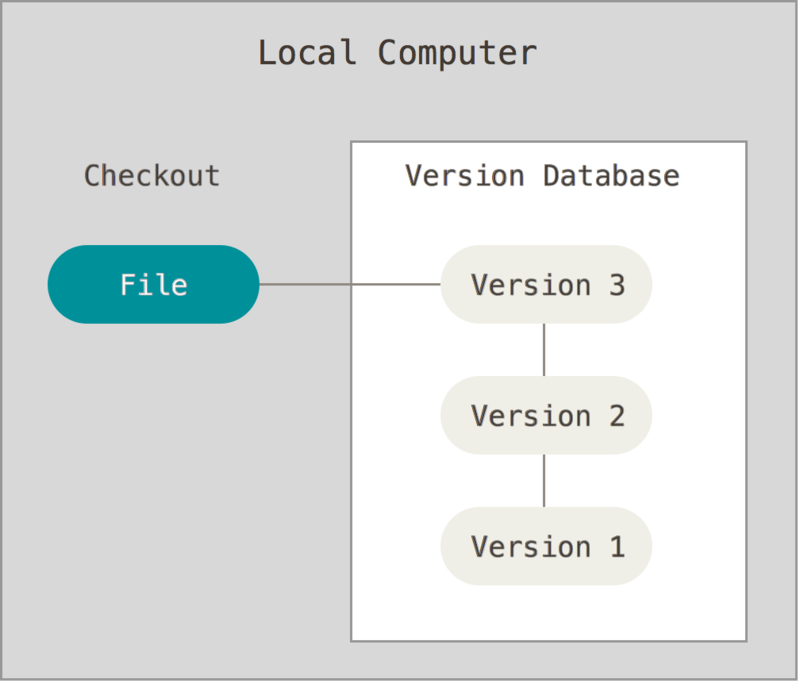
\includegraphics[height=2.75in]{../images/02-getting-started/local}
  \end{center}
\end{frame}

\begin{frame}[t]{Centralized Version Control Systems}
  \begin{center}
    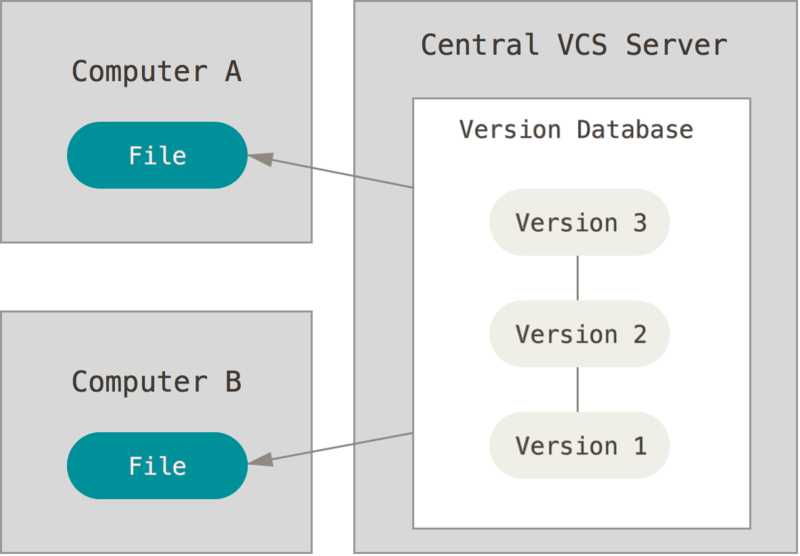
\includegraphics[height=2.75in]{../images/02-getting-started/centralized}
  \end{center}
\end{frame}

\begin{frame}[t]{Distributed Version Control Systems}
  \begin{center}
    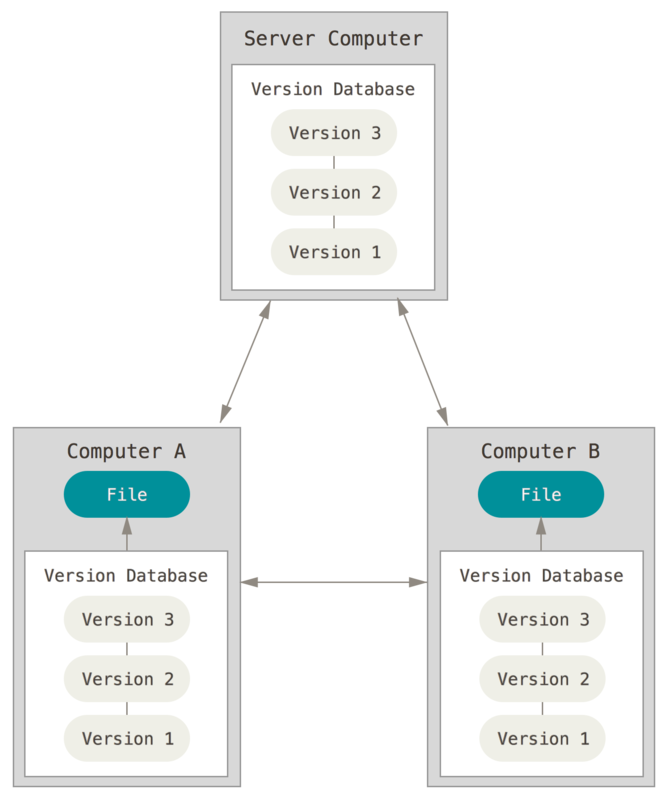
\includegraphics[height=2.75in]{../images/02-getting-started/distributed}
  \end{center}
\end{frame}

\subsection{A Short History of Git}
\begin{frame}[t]{Short History of Git}
  \begin{itemize}
    \item Linux (Linus Torvalds) vs BitKeeper
    \item 2005: Linux development community sets out to develop their own DVCS
      with goals for the new system of
      \begin{itemize}
        \item speed,
        \item simple design,
        \item strong support for non-linear development (thousands of parallel
          branches),
        \item fully distributed, and
        \item albe to handle large projects, like the Linux kernel,
          efficiently.
      \end{itemize}
  \end{itemize}
\end{frame}

\subsection{Git Basics}
\begin{frame}[t,allowframebreaks]{Snapshots, Not Differences}

  The Subversion model: file-based changes.

  \begin{center}
    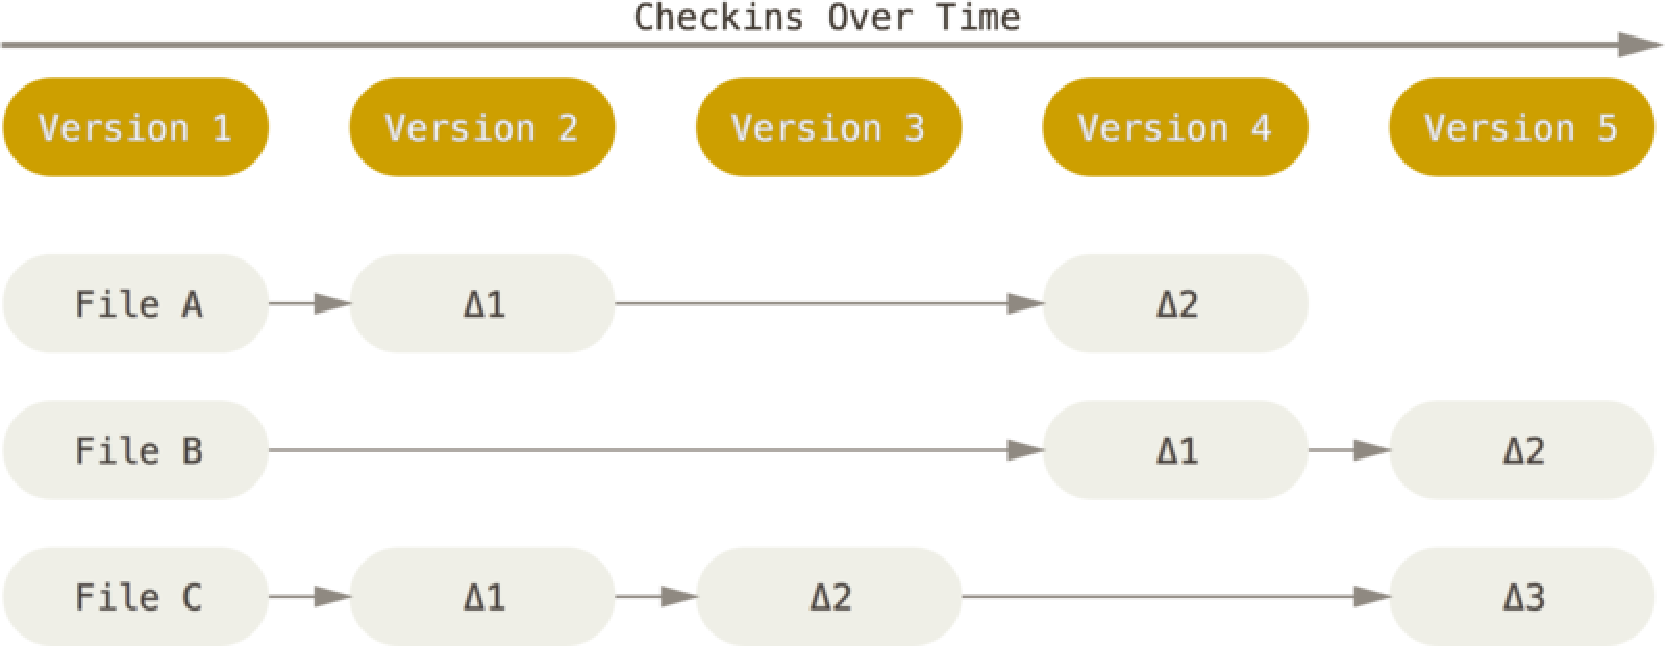
\includegraphics[width=0.98\textwidth]{../images/02-getting-started/deltas}
  \end{center}

  \pagebreak

  The Git model: a stream of snapshots.

  \begin{center}
    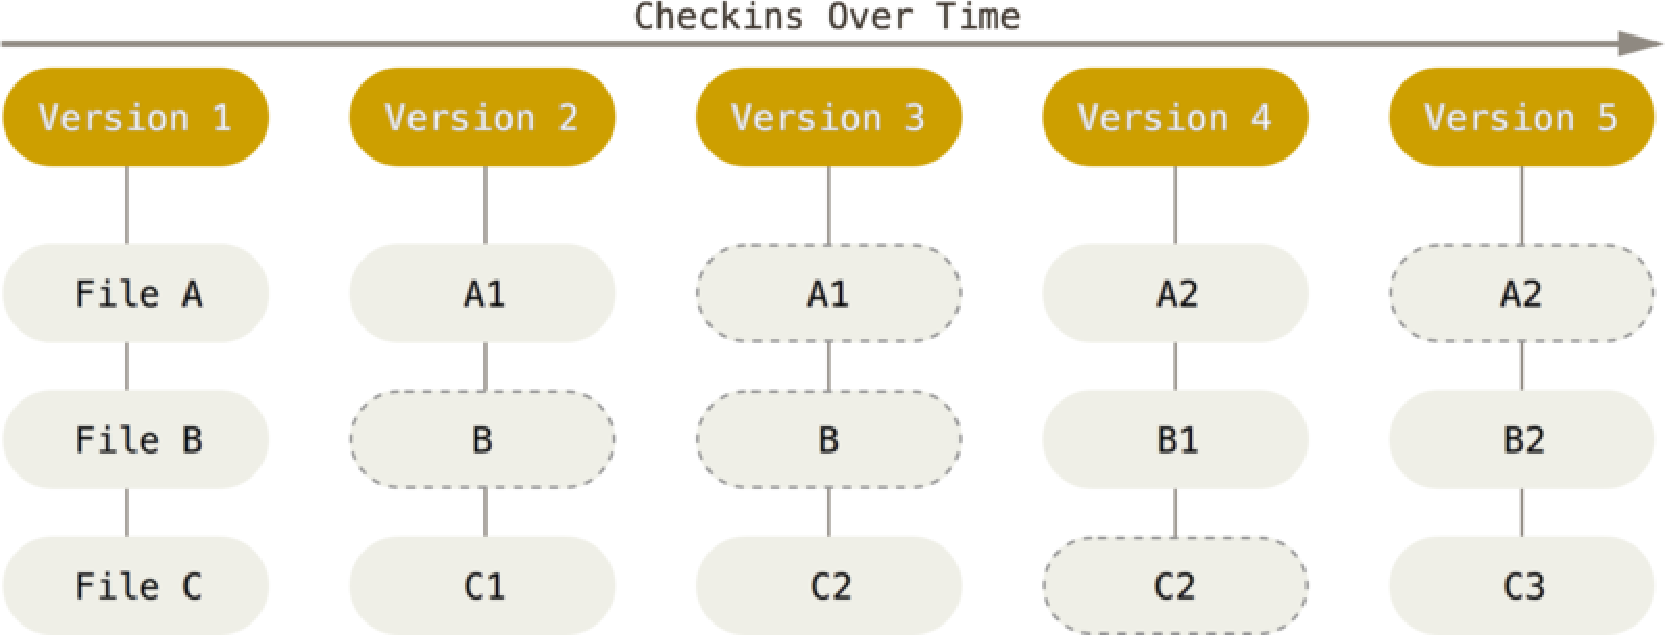
\includegraphics[width=0.98\textwidth]{../images/02-getting-started/snapshots}
  \end{center}

\end{frame}

\begin{frame}[t]{Nearly Every Operation is Local}
  \begin{itemize}
    \item Most operations are local.
      \begin{itemize}
        \item No need to talk to other computers on a network.
        \item The entire project history is on your local disk.
      \end{itemize}

    \item You can work offline.
    \item You can work off VPN.  
  \end{itemize}
\end{frame}

\begin{frame}[t]{Git Has Integrity}
  \begin{itemize}
    \item Everything is check-summed (remember the sha?)
    \item You can't lose informatin in transit nor get a file corruption without
      Git being able to detect it.
    \item Git stores everything in its database not by file name but by the hash
      value of its contents.
  \end{itemize}
\end{frame}

\begin{frame}[t]{Git Generally Only Adds Data}
  \begin{itemize}
    \item Nearly all actions in Git add data to the Git database.
    \item It is difficult to do anything that is not undoable.
    \item You can lose/corupt un-committed changes.
    \item It is very difficult to lose anything after a commit, especially with
      frequent pushes to other repositories.
  \end{itemize}
\end{frame}

\begin{frame}[t,allowframebreaks]{The Three States}
  %This is the main thing to remember about Git if you want the rest of your
  %learning process to go smoothly.  
  Git has three main states that files reside in.

  \begin{enumerate}
    \item Committed
      \begin{itemize}
        \item data is safely stored in the local database.
      \end{itemize}
    \item Modified
      \begin{itemize}
        \item changed the file(s) but have not committed to the database yet.
      \end{itemize}
    \item Staged
      \begin{itemize}
        \item Marked modified file(s) in its current version to go into the next
          commit snapshot.
      \end{itemize}
  \end{enumerate}

  This leads to three main sections of a Git project:
  \begin{enumerate}
    \item the Git directory,
    \item the working directory, and
    \item the staging area.
  \end{enumerate}

  \pagebreak

  \begin{center}
    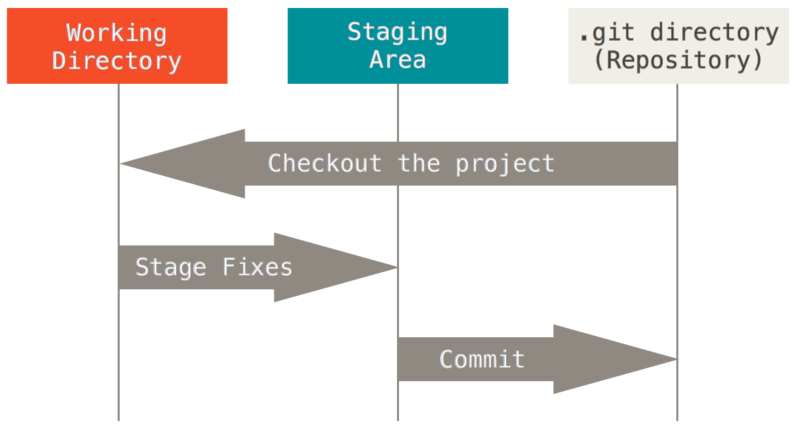
\includegraphics[height=1.55in]{../images/02-getting-started/areas}
  \end{center}

  Basic Git workflow:
  \begin{enumerate}
    \item Modify files in working directory.
    \item Stage files, adding snapshots of them to staging area.
    \item Commit.  Takes the files as they are in the staging area and stores
      that snapshot permanently in your Git directory.
  \end{enumerate} 
\end{frame}

\subsection{The Command Line}
\begin{frame}[t]{Different ways to use Git}
  \begin{itemize}
    \item Original command line tools.
    \item Many graphical user interfaces (GUIs) with verying capabilities.

    \item Command line allows you to use {\bf all} Git commands.
    \item GUIs allow for only a subset of Git commands.

    \item After install, on Windows, Mac OSx, or Linux, command line will be
      available.
    \item GUIs, take your pick. \url{http://git-scm.com/downloads/guis} has 12
      differnt GUIs with different features, OS requirments, \ldots, surely
      dozens of others exist too.
    \item RStudio has a built in Git GUI.
  \end{itemize}
\end{frame}

\subsection{Intalling Git}
\begin{frame}[t]{Git is Free!}
  \begin{itemize}
    \item Linux: install via 
      \begin{itemize}
        \item {\tt yum install git}, or
        \item {\tt apt-get install git}.
      \end{itemize}
    \item Mac: Xcode Command Lines Tools.
    \item Windows: \url{http://git-scm.com/download/win}
    \item Install form source too, if you want.
  \end{itemize}
\end{frame}

\begin{frame}[t]{Set up}
  Need to run this once after install.  Done via command line, can be done in
  {\it some} GUIs.

  {\tt
    \$ git config --global user.name "Peter DeWitt"

    \$ git config --global user.email "peter.dewitt@ucdenver.edu" 
  } 
\end{frame}

\begin{frame}[t]{Getting Help}
  You can get information on Git verbs in the terminal via:

  {\tt
    \$ git help $<$verb$>$

    \$ git $<$verb$>$ --help

    \$ man git-$<$verb$>$ 
  } 
\end{frame}
